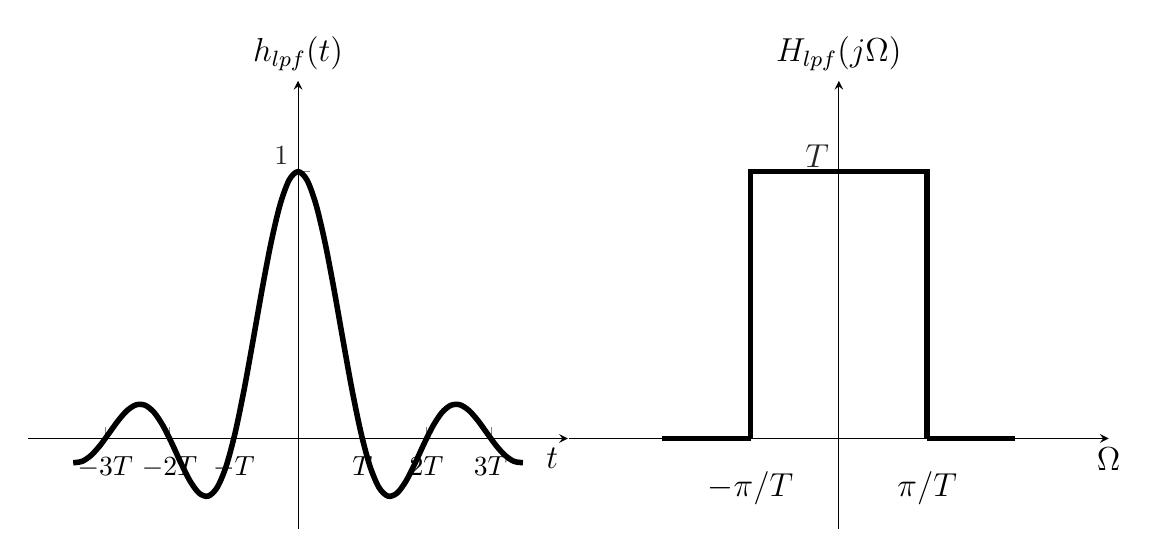
\begin{tikzpicture} 
\begin{axis}[
	name=ideal_lpf_td,
	anchor=origin,
	axis lines*=middle,
	enlargelimits = true,
	ymin=-0.2,
	ymax=1.2,
	xmin=-3.5,
	xmax=3.5,
	axis line style={->,>=stealth},
	xlabel={\large $t$},
	ylabel={\large $h_{lpf}(t)$},
	yticklabel style = {yshift=0.2cm},
	xticklabel style = {yshift=-0.1cm},
	every axis x label/.style={
		at={(ticklabel* cs:1)},
		anchor=north,
	   xshift=-0.2cm,
	},
	every axis y label/.style={
		at={(ticklabel* cs:1)},
		anchor=south,
	},
	ytick={1},
	xtick={-3, -2, -1, 1, 2, 3},
	xticklabels={$-3T$, $-2T$, $-T$, $T$, $2T$, $3T$},
	every outer y axis line/.append style={white!15!black},
	every y tick label/.append style={font=\color{white!15!black}},
	legend style={draw=white!15!black,fill=white,legend cell align=left}]
	
	\addplot[smooth, black, line width=2pt, domain=-3.5:3.5, samples=51] {sin(deg(pi*x))/(pi*x) + (x == 0)};
\end{axis}

\begin{axis}[
	name=ideal_lpf_fd,
	at=(ideal_lpf_td.right of south east), anchor=left of south west,
	axis lines*=middle,
	enlargelimits = true,
	xmax=4,
	xmin=-4,
	ymin=-0.2,
	ymax=1.2,
	axis line style={->,>=stealth},
	xlabel={\large $\Omega$},
	ylabel={\large $H_{lpf}(j\Omega)$},
	yticklabel style = {yshift=0.2cm},
	xticklabel style = {yshift=-0.3cm},
	every axis x label/.style={
	    at={(ticklabel* cs:1)},
	    anchor=north,
	},
	every axis y label/.style={
	    at={(ticklabel* cs:1)},
	    anchor=south,
	},
	ytick={1},
	yticklabels={\large $T$},
	xtick={-1.5708, 1.5708},
	xticklabels={\large $-\pi/T$, \large $\pi/T$},
	every outer y axis line/.append style={white!15!black},
	every y tick label/.append style={font=\color{white!15!black}},
	legend style={draw=white!15!black,fill=white,legend cell align=left}]

	\addplot[black, domain=-pi/2:pi/2, samples=2,line width=2pt] {1};
	\addplot[black, line width=2pt] coordinates {(-pi/2, 0) (-pi/2, 1.01)};
	\addplot[black, domain=-pi:-pi/2, samples=2,line width=2pt] {0};
	\addplot[black, domain=pi/2:pi, samples=2,line width=2pt] {0};
	\addplot[black, line width=2pt] coordinates {(pi/2, 0) (pi/2, 1.01)};
\end{axis}

\end{tikzpicture}